\documentclass[fleqn]{article}
\usepackage[utf8]{inputenc}
\usepackage{geometry}
\geometry{height=9.8in,margin={3cm,3cm}}

% --- Title Page Block --- %
\title{Gulf of Mexico - Seismic Project}
\author{
    W. Ayyad,
    E. Collins,
    K. Helland-Hansen,
    T. Singleton
}

% --- Equation Packages --- %
\usepackage{amssymb, mathtools, gensymb, amsmath, nccmath}

% --- Bib Resources --- %
\usepackage[backend=biber,style=ieee]{biblatex}
\addbibresource{./sources.bib}

% --- Images --- %
\usepackage{graphicx, float, wrapfig}
\usepackage[caption = false]{subfig}

% --- Flow Chart --- %
\usepackage{tikz}
\usetikzlibrary{matrix,shapes,arrows,positioning,chains}

% --- Tables --- %
\usepackage{tabularx, caption, booktabs, array, ragged2e, changepage, caption}
\captionsetup[table]{skip=-1em}
\renewcommand{\arraystretch}{1.2}
\newcolumntype{C}{>{\hspace{0pt}\Centering\arraybackslash}X}
\newcolumntype{L}{>{\hspace{0pt}\raggedright\arraybackslash}X}

\begin{document}

\maketitle
\tableofcontents
\pagebreak
% --- Abstract --- %
\section{Executive Summary}
In this report we present our interpretation of the Mars/Ursa field complex in the Gulf of Mexico. We processed post-stack seismic data (G3D1304-002 survey) using Petrel to identify potential reservoirs within the study region. We conducted a rock physics analysis in combination of our geological interpretation and well logs to decide horizons of interest which are prospective for oil. We then mapped a series of volumetric attributes to realize the study area. Using these attributes we found two prospective locations (Prospect A and B). Our team proposes drilling at site A (31920, 3080), and B (32920, 2900). For Prospect A we estimate our P90, P50, and P10 values as 6.7 million STB, 11.2 million STB, and 17.6 million STB. Prospect B results are 7.7 million STB, 13.2 million STB, and 20.4 million STB. 

% --- Brief Geologic Background --- %
\section{Geologic History and Petroleum Systems}

\subsection{Geological Setting}

The Gulf of Mexico (GOM) basin began forming during the Late Triassic to Early Triassic Periods during the breakup of the Pangea supercontinent, producing North East - South West trending rifts offset by North West - South East trending transfer faults throughout the region \cite{Nixon}. A rift that developed during the Middle Jurassic produced an oceanic spreading center in the region lasting approximately 10 million years \cite{Bouroullec}. The tectonic evolution of this region allowed for post-rift subsidence, and produced a Significant effects on the structural evolution of the GOM basin \cite{Bouroullec}. The Mars/Ursa geologic complex lies within this basin and is a well-known region for prolific oil and gas reservoirs. The region has experienced multiple periods of evaporite deposition followed by depositions of carbonates, siliciclastic sands, and shale. The deposition of the Louann Salt occurred during the Middle Jurassic, followed by the deposition of organic-rich carbonate mudstone during the Late Jurassic which is often noted as a major hydrocarbon source rock for the GOM \cite{Nixon}. Three other levels of allochthonous salt were deposited within the Cretaceous and Cenozoic Periods as shown in Figure \ref{fig:PetroleumSystem}. Evidence of paleo-delta systems is also preserved in the Gulf of Mexico. These delta systems originated off the coast of present-day Mississippi and deposited sand-rich sediments in the region. Throughout time these depocenters shifted from west to east and prograded from north to south due to sea level fluctuations. 

\begin{figure}[H]
    \centering
    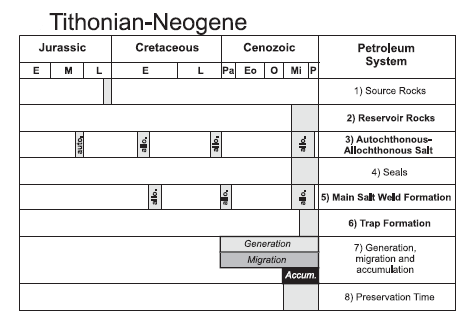
\includegraphics[width=4in]{Images/petroleum_system.png}
    \caption{A Tithonian-Neogene petroleum system element chart for the Gulf of Mexico \cite{Bouroullec}. }
    \label{fig:PetroleumSystem}
\end{figure}

\subsection{Petroleum System}
\subsubsection{Traps}
Trap types observed in the region include primarily combined structural, stratigraphic traps, and stratigraphic traps with three-way. These three-way closures are observed through fault-bounded traps, suprasalt traps against salt flanks, and subsalt traps against base salt. Fault-bounded traps often form in extensional and contractional settings, or due to regional deformation of salt. Suprasalt traps show reservoirs pinching out against the flanks of salt features while subsalt traps show reservoirs pinching out away from the base of salts \cite{Bouroullec}. Stratigraphic traps are formed where sediments pinch out and updip, primarily forming on the basinward side of salt features \cite{Bouroullec}. “Turtle” structures, which form an inverted sediment pile anticline during the collapse of minibasin flanks, are also noted within the GOM by \citeauthor{Bouroullec}. 

\subsubsection{Source Rock}
From the Tithonian-Neogene timeline, Figure \ref{fig:PetroleumSystem} provided by \citeauthor{Bouroullec}, source rocks formed during Late Jurassic while reservoir rocks, seals, and trap formation occurred during the Miocene. Carbonates and shales are noted as source rocks for hydrocarbon generation near shallower regions of the GOM \cite{Priest}. Based on other exploration projects in the Mars/Ursa region, reservoir formations are predicted to be high porosity, coarse-grained sands.

\subsubsection{Reservoirs}
Siliciclastic sediment deposited from the proto-Mississippi River during the Miocene and Pliocene epochs is noted as the major reservoir rock from which hydrocarbons migrated to \cite{Priest}. Deformation of salt within the GOM caused overlying sandstones to subside and previously mentioned traps to form. These reservoirs are often tightly sealed below layers of dense mud \cite{Priest}.

% --- Available Data --- %
\section{Available Data}
\subsection{3D Seismic Survey}
In order to pick the best structural trap, and to understand the regional topography and geometry in the Gulf of Mexico, we utilized the provided 3D seismic data volume (G3D1304-002). The location and extent of this volume are shown in Figure \ref{fig:LocationMap}, off the southeastern coast of Mississippi. The 3D seismic volume contains post-stack data including both zero and minimum phases. The seismic data analyses performed in this project are conducted using the software Petrel produced by Schlumberger.

\begin{figure}[H]
    \centering
    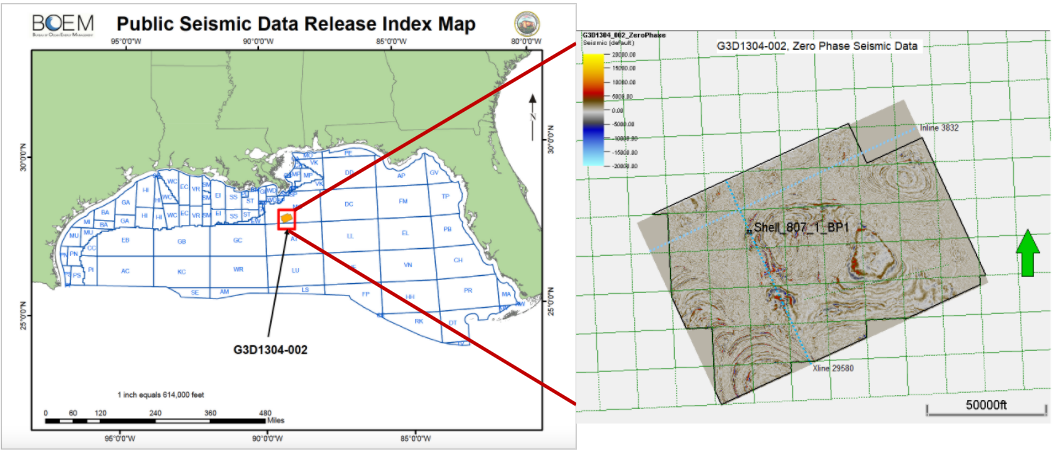
\includegraphics[width=4in]{Images/locationmap.png}
    \caption{Regional location map (left) provided by \citeauthor{BOEM}. Inset map of G3D1304-002 seismic survey outline overlain with zero phase seismic data. Shell-807 represents the well with digital logs.}
    \label{fig:LocationMap}
\end{figure}

\subsection{Wells}

The one well with digital logs available for this project is Shell\_807\_1\_BP1. The location of the well is shown in Figure \ref{fig:LocationMap}. This well provides velocity (DTC), gamma-ray (GR), density (RHOB), and porosity (PHIT) logs, which are used for seismic calibration and reservoir properties investigation. In addition, this well includes the identification of ten horizon tops. From top to bottom, the horizons identified in this well include Water bottom, Dark Red, Tan, Grey, Green, Orange, Cyan, Purple, Yellow, and Blue. Further, a checkshot (\_CPT\_Prime/DTC\_CPT) with the key well data and a velocity model are provided.

% --- Meat and Potatoes --- %
\section{Interpretation}
\subsection{Seismic-well tie}

A seismic-well tie is essential in accurately interpreting the seismic data and converting  cross-sections from two-way time (TWT) to depth. To complete the tie, the velocity (DTC) and density (RHOB) logs are used to compute impedance changes with depth. Reflection coefficients are calculated from impedance and convolved with an analytical Ricker wavelet to produce a synthetic seismogram. In Petrel, horizon tops are snapped to either peaks or troughs by comparing the synthetic seismogram and zero phase seismic data. In the ideal case, the tie would produce similar output interval velocities. 

In this project, one key well (Shell\_807\_1\_BP1) is used for seismic calibration. Figure \ref{fig:WellTie} shows the well-tie with the logs, seismic section at the well location, and the cross-correlation log. The cross-correlation presents a high percentage (60\%) correlation between the generated synthetics and seismic data. 

The ten provided well tops are identified as tops or peaks and tied to the seismic data using the generated synthetics. The water bottom, Green, Blue, and Dark Red horizons were adjusted to increase the accuracy of our tie.

\begin{figure}[H]
    \centering
    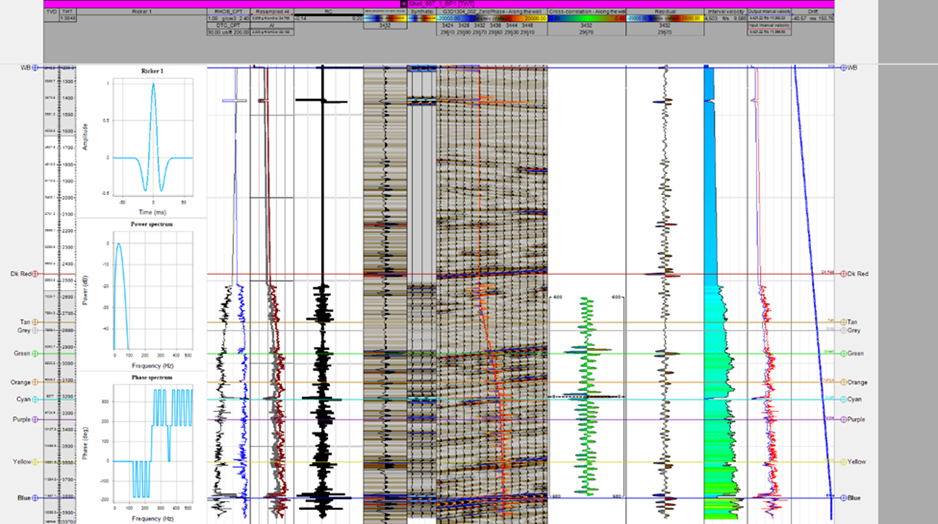
\includegraphics[width=0.75\textwidth]{Images/WellTie Extended.png}
    \caption{This figure is representative of the our method to correlate the seismic two-way-time (TWT) to distance. Using the log attributes we are able to identify corrections along the synthetic seismic generated by our Ricker wavelet. Petrel allows us to shift the synthetic seismic profile to better correlate with our data set. We are then able to transform TWT to depth.}
    \label{fig:WellTie}
\end{figure}

\subsection{Thickness Maps}

Thickness maps are generated between two horizon surfaces using the provided velocity model to convert this map from time domain to depth.  Figure \ref{fig:ThicknessMaps} shows the thickness map between the Yellow and Blue surfaces. The area in the middle of the map was removed due to the uplifting salt dome, where the seismic volume lacks good signals’ continuity and horizons are not possible to be interpreted. As illustrated, thicker zones are located at the southeastern and north regions of the map. The thickness decreases moving from the northeast to southwest and ranges on average between $\approx 600 - 1000 (ft)$.

Figure \ref{fig:ThicknessMaps} also shows the thickness map between the Orange and Yellow surfaces. Since the Purple horizon is not interpreted by the team due to its weak signal amplitudes on the seismic volume, this thickness map is generated using the closest mapped surface (Orange surface). In turn, showing a very thick interval. As illustrated, thicker zones are located at the eastern southeastern regions of the map. The thickness decreases moving from the northeast to southwest and ranges on average between $\approx 1200 - 2200 (ft)$. Both formations demonstrate good ranges of thickness and  reservoir qualities.

\begin{figure}[H]
    \centering
    \subfloat{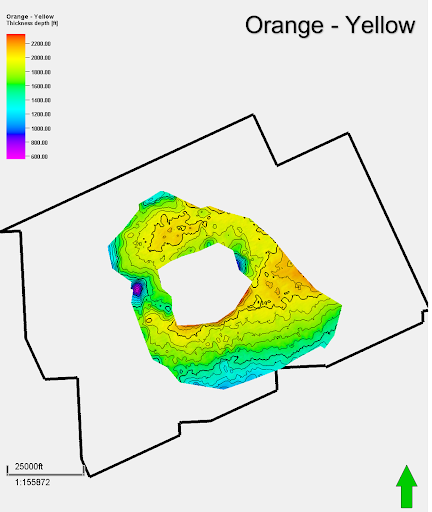
\includegraphics[width=0.48\textwidth]{Images/Orange-Yellow Thickness.png}} 
    \subfloat{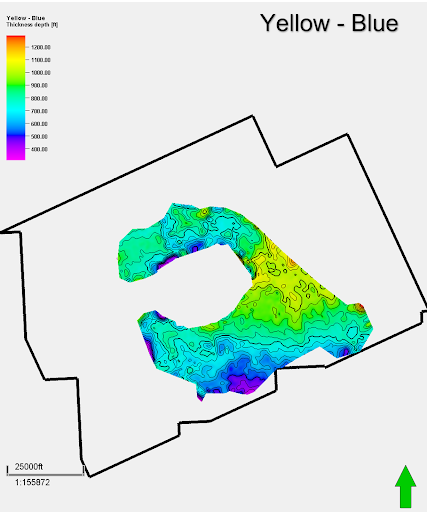
\includegraphics[width=0.48\textwidth]{Images/Yellow-Blue Thickness.png}}
    \caption{This figure shows thickness maps between the Orange-Yellow surfaces and between the Yellow-Blue surfaces.}
    \label{fig:ThicknessMaps}
\end{figure}

% --- Rock physics --- %
\subsection{Rock Physics Analysis}
Well logs analysis is one of the fundamental steps in identifying properties of the subsurface layers. It is conducted by cross-plotting the various logs at different depths. These plots are used to further identify the characteristics of the given reservoirs, including lithology, and porous zones. Compressional waves are the first to arrive at the receiver, and are able to propagate through solids and liquids in the subsurface. Arrival times are used to compute the compressional velocity (Vp) log, which is calculated using the DTC\_CPT log through the following equation, where DTC\_CPT is the measurement in ft/sec. 

\begin{ceqn}
    \begin{equation} \label{eq:CompressionalVelocity}
        \centering
        V_p\frac{m}{s} = \frac{304800}{DTC\_CPT}
    \end{equation}
\end{ceqn}

Therefore, Vp is sensitive to the existing liquids and pores spaces in the reservoir rocks, which is illustrated by a relative decrease. Vp increases as a response to compacted, and less porous rocks. The gamma ray (GR) log is used to identify the lithology, specifically, high shale zones. High GR values are an indication of a high volume of shale in a sand-shale interval. The decrease in shale volume corresponds to lower GR values and a cleaner sand interval. Furthermore, the volume of shale is determined by using the gamma ray (GR\_CPT) log as an input in the following equation:

\begin{ceqn}
    \begin{equation} \label{eq:Vshale}
        \centering
        V_{shale}(\%) = \frac{GR_{CPT}-GR_{min}}{GR_{max} - GR_{min}}
    \end{equation}
\end{ceqn}

The density log (RHOB\_CPT) provides density values in (g/cc) for rocks at different depths. Good quality reservoir intervals typically demonstrate lower density values. Density logs are generally used to calculate porosity. The total porosity (PHIT\_CPT) estimates the porous zones relative to other intervals. Measured and calculated logs are presented in Figure \ref{fig:UpperLower}. The acoustic impedance (AI) log is calculated by multiplying the RHOB\_CPT and Vp logs, and in turn, is affected by both properties. This physical property describes the resistance encountered by the propagating wave.

The well interval is divided into two based on GR log. The upper and lower section are cross-plotted using AI versus PHIT colored by $V_{shale}$ (Figure \ref{fig:UpperLowerCrossplot}). Most of the points corresponding to the upper section feature higher $V_{shale}$ values corresponding to lower porosities and higher densities compared to the lower section. The low $V_{shale}$ points with high PHIT and low AI correspond to the top three shallow intervals (Figure), which demonstrate thin layers of porous sand in alternating shale/mud and sand sequences. Generally, the lower section of the well includes thick and relatively porous intervals with low AI and $V_{shale}$ (Figure), which demonstrate good reservoir properties. These intervals are better analyzed and viewed on cross plots as the lower section is divided into the Purple, Yellow, and Blue formations.

\begin{figure}[H]
    \centering
    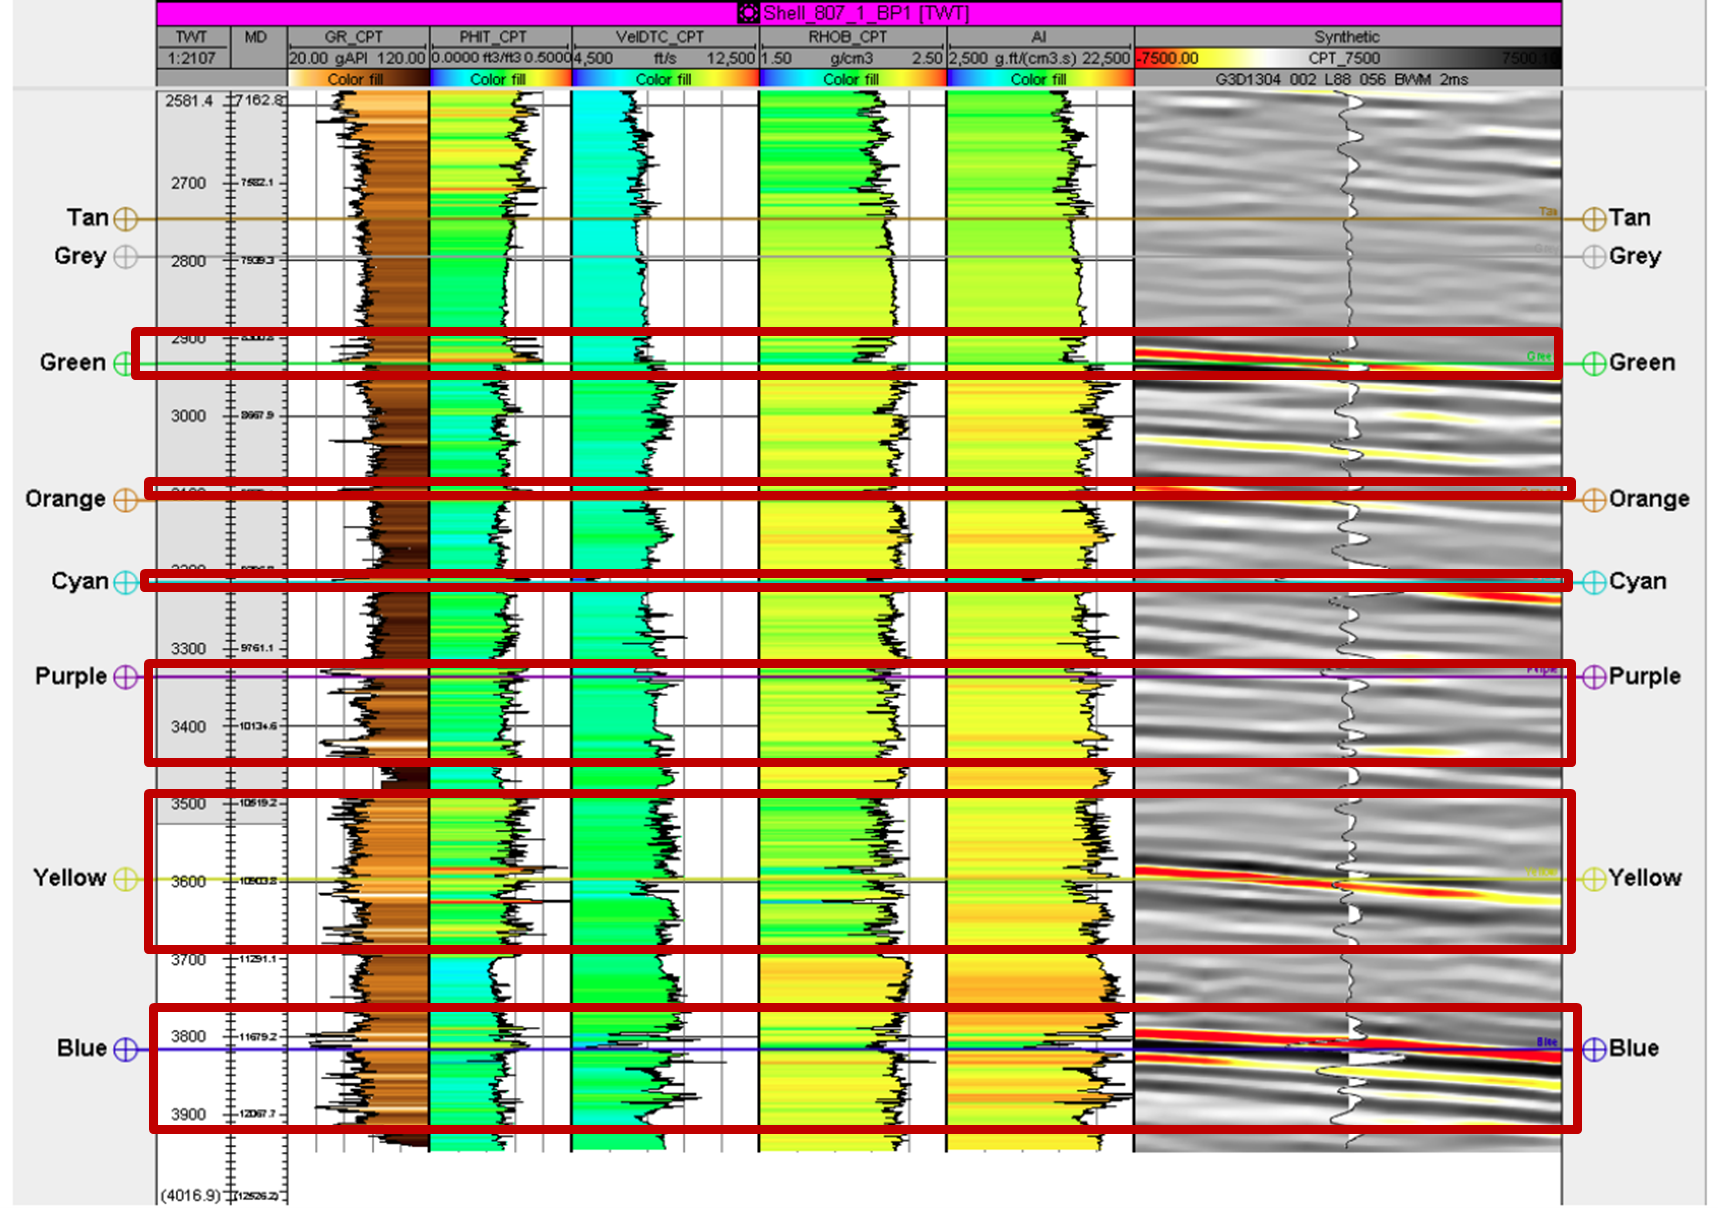
\includegraphics[width=0.9\textwidth]{Images/UpperAndLower.png}
    \caption{This figure shows the Upper and Lower sections of the well. Highlighted in red are the good sand reservoir intervals.}
    \label{fig:UpperLower}
\end{figure}

From Figure \ref{fig:UpperLower}, the Purple formation logs show a high $V_{shale}$ interval with low porosity and high AI points, which corresponds to the high GR interval located between the upper and lower clean sands. However, less $V_{shale}$ and lower AI values reflect the upper and lower sections of the Purple formation. The Yellow formation contains relatively less shale volume compared to the Purple and Blue formations with good reservoir qualities presented in high porosities, low AI and $V_{shale}$ values. The Blue formation contains a low volume of shale that increases at the bottom of the formation in addition to low AI and high PHIT values for most of the points.

\begin{figure}[H]
    \centering
    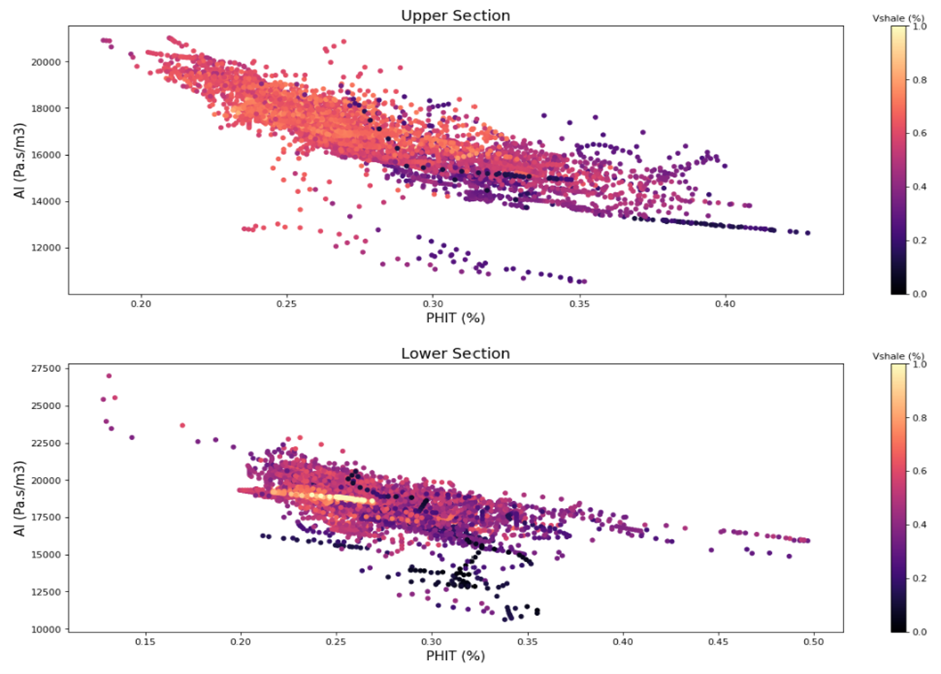
\includegraphics[width=0.9\textwidth]{Images/UpperAndLowerCrossplot.png}
    \caption{This figure shows a cross-plot of AI versus PHIT colored in $V_{shale}$ for the Upper and Lower sections of the well interval.}
    \label{fig:UpperLowerCrossplot}
\end{figure}

From Figure \ref{fig:FormationCrossPlots}, the Purple formation logs show a high $V_{shale}$ interval with low porosity and high AI points, which corresponds to the high GR interval located between the upper and lower clean sands. However, less $V_{shale}$ and lower AI values reflect the upper and lower sections of the Purple formation. The Yellow formation contains relatively less shale volume compared to the Purple and Blue formations with good reservoir qualities presented in high porosities, low AI and $V_{shale}$ values. The Blue formation contains a low volume of shale that increases at the bottom of the formation in addition to low AI and high PHIT values for most of the points.

\begin{figure}[H]
    \centering
    \subfloat[Purple]{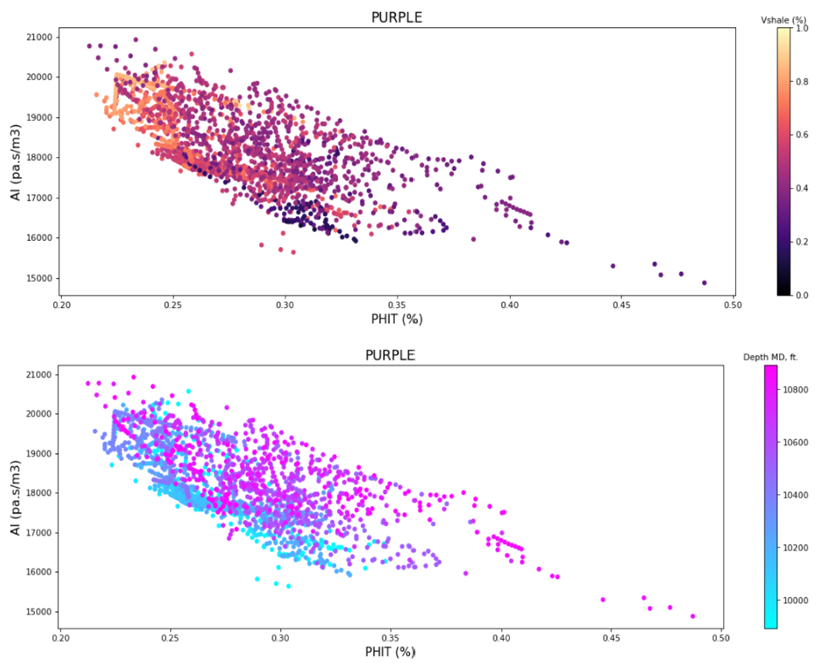
\includegraphics[width=0.48\textwidth]{Images/PurpleCrossPlot.png}} 
    \subfloat[Yellow]{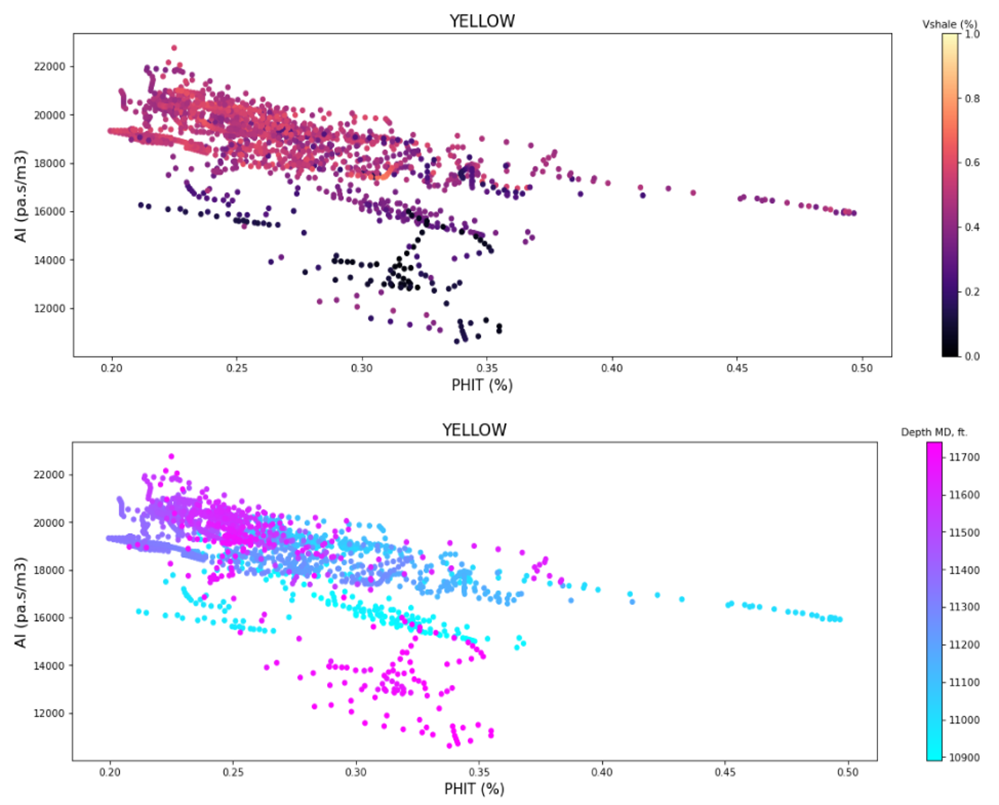
\includegraphics[width=0.48\textwidth]{Images/YellowCrossPlot.png}} \\
    \subfloat[Blue]{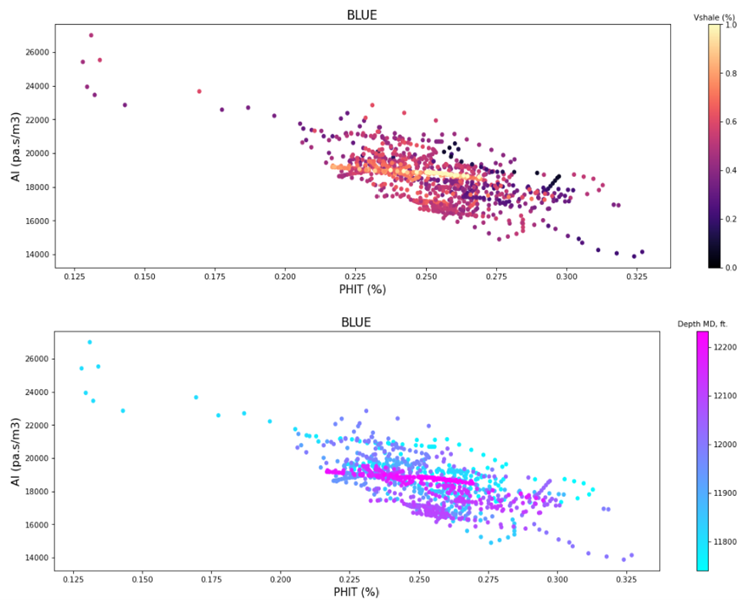
\includegraphics[width=0.48\textwidth]{Images/BlueCrossPlot.png}}
    \caption{This figure shows a cross-plot of AI versus PHIT colored in $V_{shale}$ for the Purple, Yellow, and blue formation}
    \label{fig:FormationCrossPlots}
\end{figure}

% --- Seismic QC and Tuning --- %
\subsection{Seismic Data QC and Tuning Analysis}

The wavelet was extracted from the seismic data using a statistical wavelet extraction. The extracted wavelet showed a positive polarity which is consistent with the polarity of the water bottom. Looking at the resulting power spectrums, the maximum and minimum frequencies were read to be 50 and 10Hz respectively. Using these values the Central frequency was calculated to be 30Hz. This central frequency was further used to do wedge and tuning analysis. 

Tuning analysis is done to check what the tuning thickness of the individual sands are and to gain an understanding of our seismic resolution for the different intervals. This is important to know when interpreting amplitude effects because if the sand is below tuning thickness, changes in the amplitude might be due to changes in the bed thickness and not fluid and reservoir property changes. The tuning analysis has been done using python, the input parameters are the average density and velocity of the reservoir as well as the overburden and underburden.

The tuning analysis was done on five sand intervals within the most interesting area between the purple and blue horizon. Average values for the density and velocities of the five sands were picked from the logs and can be seen in Table \ref{tab:Tuning}. Figure \ref{fig:Tuning} shows the resulting seismic wiggle graph and tuning curve plot for each sand. The red lines in the tuning curve plots indicate the thickness of the corresponding sand body. If this thickness line plots to the left of the tuning peak then the sand thickness is above tuning. As you can see sand one and two are both well above the tuning thickness. Sand three and four are just above tuning while sand five is slightly below tuning. 

\begin{figure}[H]
    \centering
    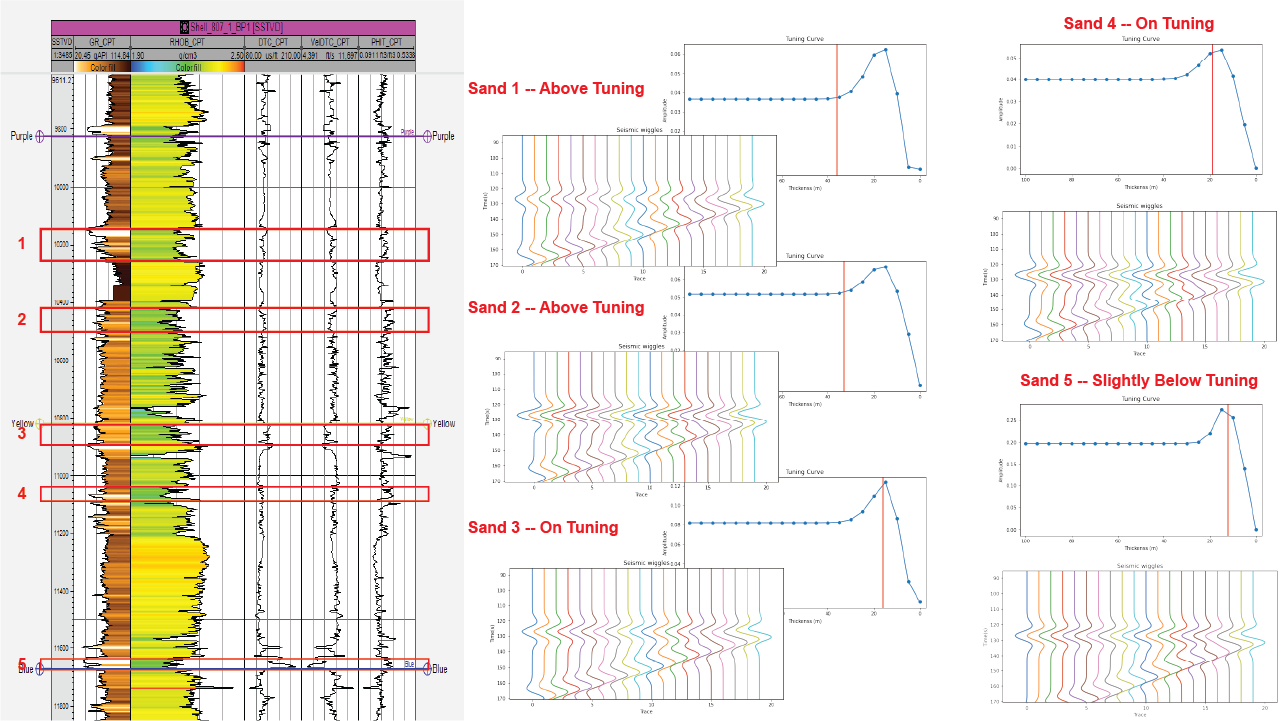
\includegraphics[width=\textwidth]{Images/Tuning.png}
    \caption{We conducted our tuning analysis within python by taking the thickness and acoustic impedance of our overburden, horizon, and underburden (Table \ref{tab:Tuning}). A synthetic seismogram was computed using our Ricker wavelet. We graphed the generated synthetic seismograph and tuning corresponding tuning curve.}
    \label{fig:Tuning}
\end{figure}

\begin{table}[H]
    \centering
    \caption{Tuning Analysis}
    \begin{adjustwidth}{-0.12\textwidth}{-0.12\textwidth}
        \begin{tabularx}{\linewidth}{@{} C *{7}{L} @{}}
    \toprule
    Sands &
    Thickness [m] & 
    Overburden Density $[cc]$ & 
    Overburden Velocity $[ms^{-1}]$ &
    Reservoir Density $[cc]$ & 
    Reservoir Velocity $[ms^{-1}]$ &
    Underburden Density $[cc]$ &
    Underburden Velocity $[ms^{-1}]$ \\
    
    \midrule
    1 & 36 & 2.24 & 2539 & 2.16 & 2433 & 2.26 & 2643 \\
    2 & 33 & 2.23 & 2591 & 2.12 & 2438 & 2.18 & 2560 \\
    3 & 16 & 2.23 & 2591 & 2.10 & 2307 & 2.24 & 2652 \\
    4 & 19 & 2.20 & 2682 & 2.09 & 2591 & 2.20 & 2637 \\
    5 & 12 & 2.24 & 2635 & 2.10 & 1829 & 2.22 & 2668 \\
    \bottomrule
\end{tabularx}
        \label{tab:Tuning}
    \end{adjustwidth}
\end{table}

% --- Attributes --- %
\subsection{Amplitude Accentuating Attribute: RMS Amplitude}

The Root Mean Square (RMS) Amplitude is calculated by taking the square root of the average of a series of squared amplitudes. This attribute sums the amplitudes in a specified window and stacks the energy to give a quick and good indicator of areas of interest. The RMS is run over a window around each horizon. To make sure that the maximum amplitude available in the wavelet is captured the window starts a quarter of a wavelength above the horizon and ends a quarter of a wavelength below the horizon. The areas in the RMS map that have the brightest amplitudes are potential areas containing hydrocarbons.

RMS surfaces were created for all the interpreted horizons. The blue and yellow surfaces were the main focus due to the reservoir properties being best in this interval. These surfaces can be seen in Figure \ref{fig:RMS}. This figure also shows the two potential prospect areas A and B. These prospects are chosen over the brightest amplitudes at the edge of the salt dome in the middle. The brightest amplitudes with the largest extent can be seen on the blue RMS surface, there are also bright amplitudes in the same locations on the yellow surface, but the amplitudes cover a smaller area.

\begin{figure}[H]
    \centering
    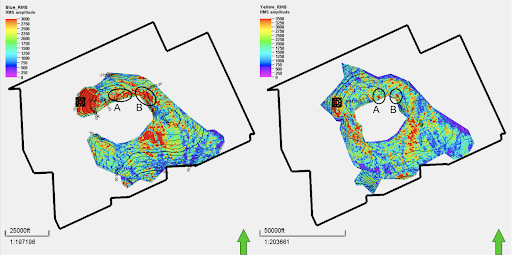
\includegraphics[width=0.9\textwidth]{Images/RMS Surfaces.png}
    \caption{The RMS amplitude for our blue horizon (left) and yellow horizon (right). Using RMS amplitude we were able to identify the extent of our prospects and locations to drill.}
    \label{fig:RMS}
\end{figure}

\subsection{Instantaneous Attributes: Quadrature and Instantaneous Phase}

The first seismic attribute computed for the seismic volume was a 90-degree phase shift, also referred to as a Poor Man’s Inversion or Quadrature. While zero-phase seismic data is often superior for interpreting simple, thick-layered systems, clarity is often lost with complex, thin-bed sections. The Poor Man’s Inversion improves the seismic interpretability of our prospect regions by eliminating the dual polarity of thin-bed responses, resulting in clearer impedance profiles \cite{Zeng}. This is shown in Figure \ref{fig:Quad} below. The instantaneous phase is implemented to highlight lateral continuity of our horizons in regions of interest (shown in Figure \ref{fig:ProspectB}). This attribute also provides visualization of sequence boundaries and bedding configurations.

\begin{figure}[H]
    \centering
    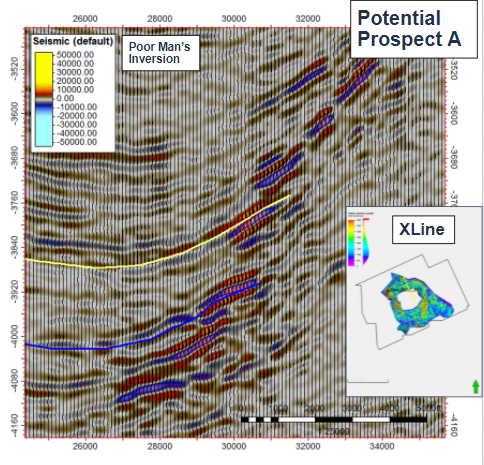
\includegraphics[width=0.9\textwidth]{Images/poor_mans.PNG}
    \caption{Quadrature for Prospect A.}
    \label{fig:Quad}
\end{figure}

\subsection{Geometric Attributes: Curvature, Ant-Tracking, and Variance}

In our geometric interpretations, we combine coherency and curvature to understand stresses and fracturing our reservoir is undergoing. Under curvature, we are interested in looking at the most positive and most negative aspects of our horizons. Anticline features are associated with positive curvature and syncline features will be associated with negative curvature. Primarily we will be viewing the curvature between our orange and yellow horizons per our geophysical analysis showcasing these sands as having significant permeability and porosity. Additionally, in reference to our geologic analysis, we are interested in the sands which reside within the early Miocene epoch which is characteristic of large clastic sedimentation from the Mississippi delta.

\begin{figure}[H]
    \centering
    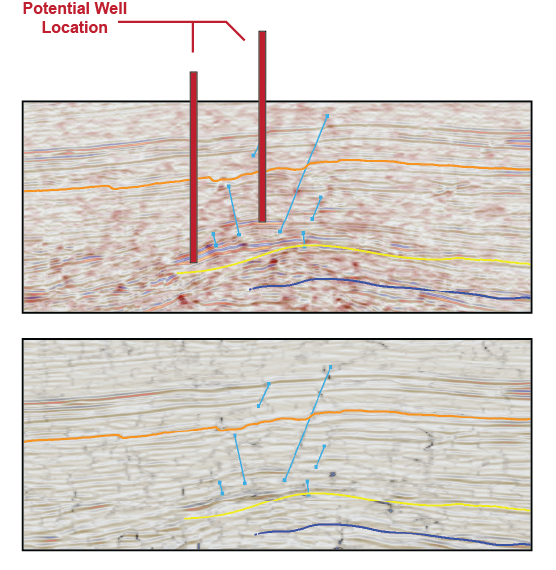
\includegraphics[width=0.9\textwidth]{Images/Curvature-Well Location.png}
    \caption{The top image in this figure shows our most positive curvature overlapped with seismic. The bottom image displays our ant-tracking with seismic. The figures were taken at Xline 32120 and Inline 3080. With a Z value of -3700.}
\label{fig:CurvatureOverlapping}
\end{figure}

Seen in our figure, we can interpolate faults inducing structural traps for our prospect by overlaying our ant-tracking with seismic and curvature attributes. Referencing our figure below our work flow for curvature and ant-tracking was based on constructing a structural smoothing filter along our seismic data profile to reduce processing time and prevent over interpretations induced from measuring and processing artifacts. Once applied, we introduced a variance attribute to highlight edge detection for ant tracking along the horizons. Our variance attribute allows us to see more subtle features in discontinuities along seismic horizons for greater understanding of the stresses close to our salt structures. Inputting the variance attribute for ant tracking, we realized to a volumetric output. Our Curvature workflow uses much the same method. We mapped curvature across our seismic profile using the structural smoothed seismic reflections. 

\begin{figure}[H]
    \begin{minipage}[b]{\textwidth}
        \centering
        % Define block styles
\tikzset{
block/.style={
    rectangle,
    draw,
    text width=0.33\textwidth,
    text centered,
    rounded corners
},
cloud/.style={
    draw,
    ellipse,
    minimum height=2em
},
descr/.style={
    fill=white,
    inner sep=2.5pt
},
connector/.style={
    -latex,
    font=\scriptsize
},
rectangle connector/.style={
    connector,
    to path={(\tikztostart) -- ++(#1,0pt) \tikztonodes |- (\tikztotarget) },
    pos=0.5
},
rectangle connector/.default=-2cm,
straight connector/.style={
    connector,
    to path=--(\tikztotarget) \tikztonodes
}
}

\begin{tikzpicture}
\matrix (m)[matrix of nodes, column  sep=2cm,row  sep=8mm, align=center, nodes={rectangle,draw, anchor=center} ]{
    |[block]| {Seismic Amplitude} \\
    |[block]| {Applied Structural Smoothing Filter} & |[block]| {Consistent Dip \\ Xline \& Inline} \\
    |[block]| {Variance Attribute (Edge Detection)} & |[block]| {Curvature Attribute \\ Most Positive \& \\ Negative} \\
    |[block]| {Ant-Tracking Attribute} \\
};
\path [>=latex,->] (m-1-1) edge (m-2-1);
\path [>=latex,->] (m-2-1) edge (m-3-1);
\path [>=latex,->] (m-3-1) edge (m-4-1);

\path [>=latex,->] (m-2-1) edge (m-2-2);
\path [>=latex,->] (m-2-2) edge (m-3-2);

\end{tikzpicture}


        \caption{A structural filter was applied to our seismic profile to reduce processing load and post-processing artifacts within the final ant-tracking model. Additionally, our smoothed seismic profile was used to process our curvature cube which required a high resolution cross-line (xline) and inline attribute to realize. We used Petrel's consistent dip model to produce these inputs.}
        \label{fig:Curvature_Flowchart}
    \end{minipage}
\end{figure}

As expected, our curvature becomes more intense when approaching the surrounding salt structure. When overlapped with ant-tracking, faults become more apparent. By overlapping curvature with ant-tracking and seismic reflections, we further reduce over interpretation and map out faulting which most appropriately align to the seismic and geological interpretation.

In our prospect, we see a structural trap formed from the salt dome intruding into the horizons. The stress caused the overburden rock to fracture which trapped the oil migrating along our salt and into our horizon. We see bright spots along the horizons indicating this.

% --- Horizon interpretation --- %
\subsection{Horizon Interpretation}

The main horizons interpreted in our prospect regions were the orange, purple, yellow, and blue horizons. We found that these horizons were generally continuous and provided strong amplitude contrasts. In our interpretation process, we only mapped regions of continuity and excluded areas where horizons encountered salt structures or faults.

The orange horizon is interpreted as a peak through the given seismic volume. The relatively strong reflector occurs because AI increases moving from the Green to the Orange formation. This horizon shows good continuity with moderately high amplitudes in the middle of the seismic volume. The yellow horizon is interpreted as a trough and the blue horizon is interpreted as a peak. Similarly to the orange horizon, both the yellow and blue tops display good continuity and strong reflectors. Outside of our prospect regions, the water bottom, red, and green horizons also display generally good continuity. While the tan, gray, and cyan horizons produce acoustic impedance contrasts, we found that these reflectors have varied continuity throughout the study region. 

% --- Fault interpretation --- %
\subsection{Fault Interpretation}

Our fault interpretations relied on picking faults that corresponded to a combination of seismic attributes. We used ant-tracking as the main component to determine their location and direction. Overlapping ant-tracking with our seismic profile, we can gather a picture of the foot and hanging walls. Finally, overlapping both attributes with variance (edge detection), we gain more insight as to where our ant-tracking attribute is detecting discontinuities. This helps us from over interpreting the more subtle discontinuities our ant-tracking attribute realizes as it is composed from our variance as discussed in section Curvature and Ant-Tracking.

% --- Reservoirs --- %
\section{Reservoirs}
\subsection{Prospect A}

Using our RMS attribute, we were able to identify initial locations with high seismic amplitude. Ensuring these amplitudes are not due to other geologic processes, we compared our map with coherency. We identified Prospect A at Xline 32200 and Inline 3080 with a depth of $-3700ft$. This reservoir has significant bright seismic reflections and flat spots giving us indications of significant hydrocarbon deposits. Viewing the coherency attribute, we can identify faulting from the stress induced by the migrating salt. This gives us a structural trap between the salt and sealed by faults. We believe the faults are sealing because the edges of our bright spots do not extend past them. Placing a well that laterally follows the salt would provide the most productive results. This is because the oil is attempting to migrate upward along the salt. Based on the thickness maps and high amplitude reflections at this location, the Yellow and Blue sands interval shows a large thickness that ranges between $\approx 600 - 700 (ft)$. According to our tuning analysis of the yellow sands, the reflections are within the tuning range, so we also trust the strong seismic reflections are not due to shallow high acoustic impedance layers or a tuning effect.

\begin{figure}[H]
    \centering
    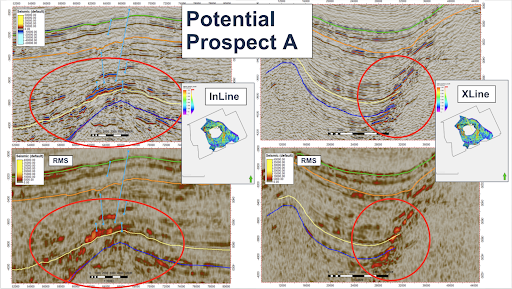
\includegraphics[width=0.9\textwidth]{Images/ProspectA.png}
    \caption{Prospect A is found at Xline 32200 and Inline 3080. The extent of the reservoir is captured using RMS amplitude which highlights the bright spots from our seismic.}
    \label{fig:ProspectA}
\end{figure}

\subsection{Prospect B}

The oil in Prospect B appears to be structurally trapped from the sands above. This seals the oil from moving further. These overburden layers are mostly composed of shale which we have identified in the rock physics section and view along the well logs. Prospect B does not display any significant faulting. As with Prospect A, Prospect B is within tuning, so we can trust the bright spots from our seismic profile to be representative of hydrocarbons. Based on the thickness maps and high amplitude reflections at this location, the Yellow and Blue sands interval shows a large thickness that ranges between $\approx 600 - 700 (ft)$. We place Prospect to be at a Xline 32920 and Inline 2900.

\begin{figure}[H]
    \centering
    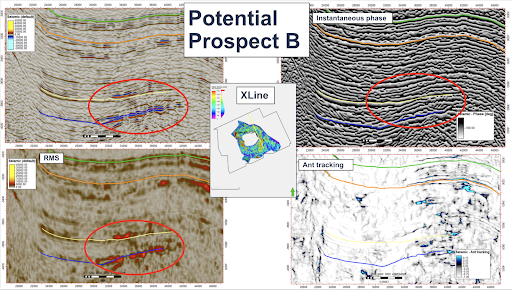
\includegraphics[width=0.9\textwidth]{Images/ProspectB.png}
    \caption{Prospect B is found at Xline 32920 and Inlin 2900. RMS amplitude helps to highlight the extent of the prospect. Instantaneous phase shows us the continuity of our horizon through the salt which we cannot see in our seismic. Ant-tracking highlights the discontinuities within the prospect.}
    \label{fig:ProspectB}
\end{figure}

% --- Reserve estimation/econ analysis --- %
\section{Reserves Estimation and Economic Analysis}
The main equations used to compute original oil in place (OOIP) and original gas in place (OGIP) are noted in the Appendix. To compute recoverable reserves, OOIP or OGIP are multiplied by the appropriate recovery factor. The recovery factor is estimated from the type of drive mechanism. For our calculations we used a drive mechanism of depletion in solution/gas, which corresponds to a recovery factor of 18-25\%. A gas-oil ratio of 1.35 Mof/bbl was taken from the Field Summary Report \cite{ESA} to determine the formation volume factors for oil. To determine the formation volume factor for gas, average reserve temperatures and pressures for the GOM are used in the equation noted in Appendix 3. A porosity of 0.3 is derived from clean sands, as identified in the Rock Physics section. Water saturation is estimated from known values in the GOM. Reservoir thicknesses and areas for each prospect are estimated using well logs and seismic data in cross section and map view. Variables and results for volumetric estimation are outlined in Table 1. Based on these calculations Prospect A has a recoverable oil volume of approximately 14.2 million bbl, and a recoverable gas volume of approximately 418,000 million cubic feet. Prospect B has slightly higher values, with a recoverable oil volume of 1.64 million bbl and a recoverable gas volume of 482,000 million cubic feet. Associated revenues for each prospect are outlined in Table \ref{tab:Prospect_Reserves} based on current average oil and gas prices in the United States. These revenues do not include total expenditures.

\begin{table}[H]
    \centering
    \caption{Prospect Economic Analysis}
    \begin{adjustwidth}{-0.12\textwidth}{-0.12\textwidth}
        \begin{tabularx}{\linewidth}{C *{8}{L}}
    \toprule
    Prospect &
    H $(ft)$ &
    A $(ac)$ &
    Boi $(\frac{bbl}{STB})$ &
    Bgi $(\frac{ft^3}{SCF})$ &
    Recov. N $(STB)$ &
    Recov. G $(SCF)$ &
    Total Oil Revenue $(USD)$ &
    Total Gas Revenue $(USD)$ \\
    
    \midrule
    A & 650 & 150 & 1.725 & 4.56$e^{-4}$ & 1.42$e^7$ & 4.18$e^{11}$ & 1.21 B & 41.76 B \\
    B & 750 & 150 & 1.725 & 4.56$e^{-4}$ & 1.64$e^7$ & 4.82$e^{11}$ & 1.39 B & 48.18 B \\
    \bottomrule
\end{tabularx}
        \label{tab:Prospect_Reserves}
    \end{adjustwidth}
\end{table}

\begin{table}[H]
    \centering
    \caption{P90, P50, P10 Volume Estimates}
    \begin{adjustwidth}{-0.12\textwidth}{-0.12\textwidth}
        \begin{tabularx}{\linewidth}{C *{8}{L}}
    \toprule
    Prospect &
    P90 (STB) &
    P50 (STB) &
    P10 (STB) &
    P90 (SCF) &
    P50 (SCF) &
    P10 (SCF) 
    \\
    
    \midrule
    A & 6.72$e^{6}$ & 11.18$e^{6}$ & 17.60$e^{6}$ & 2.44$e^{11}$ & 4.00$e^{11}$ & 6.11$e^{11}$ \\
    B & 7.66$e^{6}$ & 13.19$e^{6}$ & 20.38 $e^{6}$ & 2.89$e^{11}$ & 4.63$e^{11}$ & 7.05$e^{11}$ \\
    \bottomrule
\end{tabularx}
        \label{tab:p90}
    \end{adjustwidth}
\end{table}

% --- Risks/Pitfalls --- %
\section{Risk Analysis and Pitfalls}
\subsection{Financial Risks}
Uncertainty in reservoir properties and price of oil and gas produces a range of recoverable volumes and revenues as noted in Figure ~\ref{fig:A_prod} and ~\ref{fig:B_prod}. Our P90, P50, and P10 values for oil in Prospect A are 6.7 million STB, 11.2 million STB, and 17.6 million STB, respectively. Our P90, P50, and P10 values for Prospect B are 7.7 million STB, 13.2 million STB, and 20.4 million STB, respectively. Oil revenue can range from \$0.46 - \$1.665 billion USD for Prospect A and \$0.566 - \$2.074 billion USD for Prospect B. P90, P50, and P10 gas values for each prospect are provided in Table \ref{tab:p90}. Gas revenue can range from \$17.3 - \$80.1 billion USD for Prospect A and \$19.3 - \$90.9 billion USD for Prospect B. These ranges are primarily due to uncertainty in reservoir thickness, area, and the price of oil or gas. While there are large revenues for each prospect, the saturation of hydrocarbons is also uncertain and therefore these ranges may represent high revenue estimates. Based on production reports for MC807, average revenues for oil and gas in the Mars/Ursa field can range from roughly 4-8 million bbls or Mcf per year \cite{ESA}.

\begin{figure}[H]
    \centering
    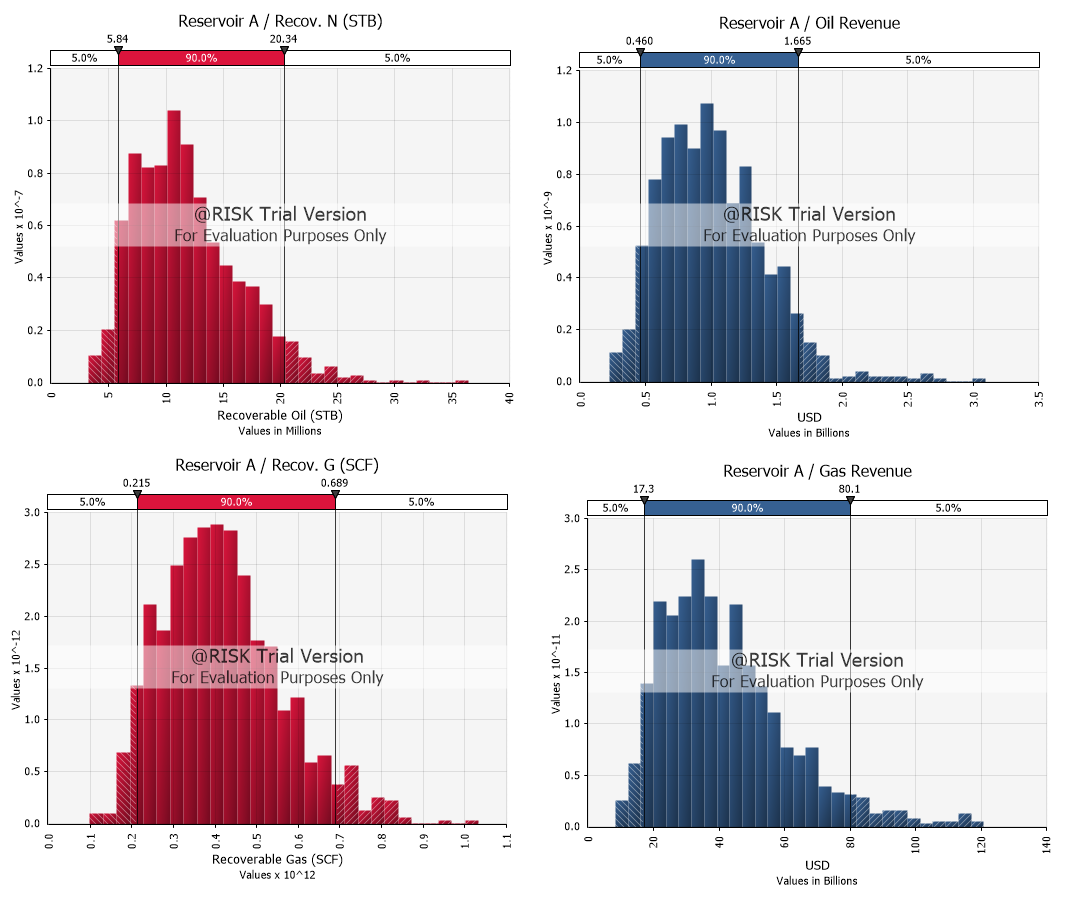
\includegraphics[height=3.5in]{Images/A_production.png}
    \caption{Risk analysis for recoverable volumes and revenues for oil and gas in Prospect A.}
    \label{fig:A_prod}
\end{figure}

\begin{figure}[H]
    \centering
    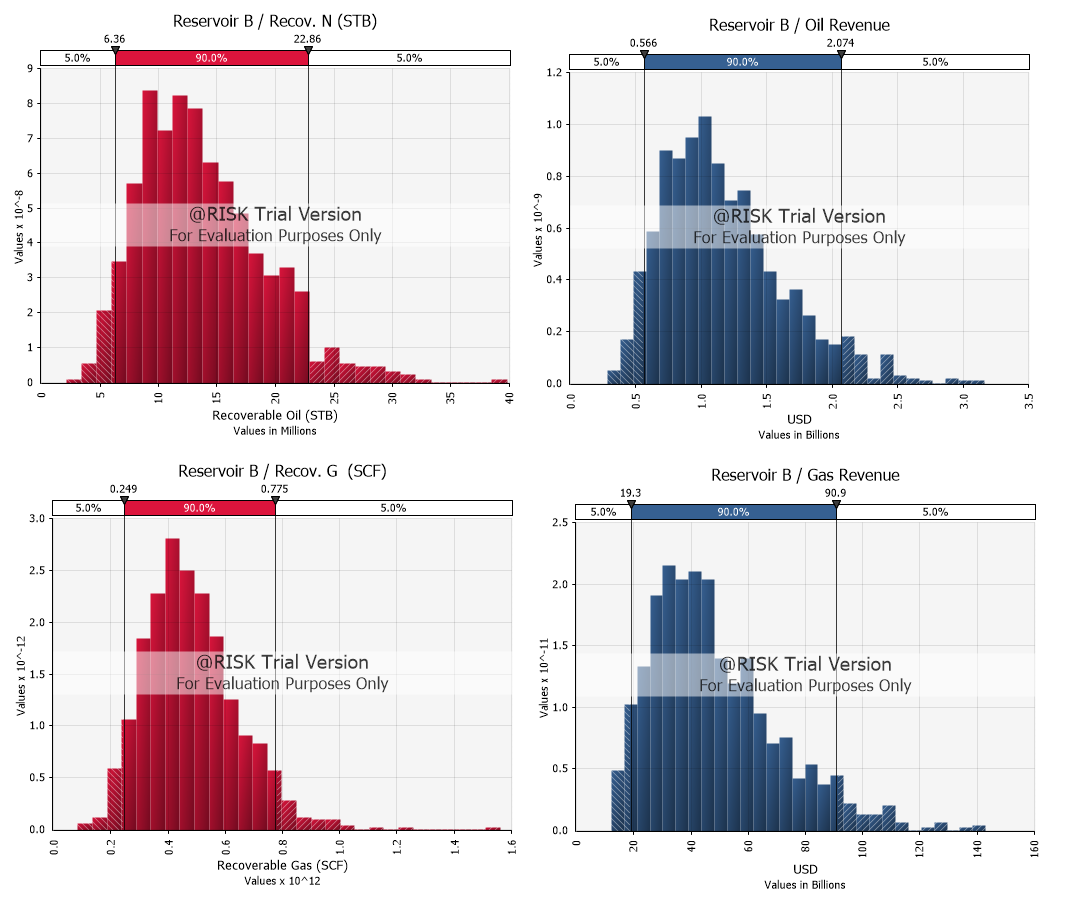
\includegraphics[height=3.5in]{Images/B_production.png}
    \caption{Risk analysis for recoverable volumes and revenues for oil and gas in Prospect B.}
    \label{fig:B_prod}
\end{figure}

\subsection{Operational Risks}
Apart from uncertainty in production volume and revenue, there are a number of common operational risks in the GOM including borehole instability, underpressured or overpressured formation zones, and unconsolidated sands. These operational risks may result in damaging the reservoir, blowouts, mud loss, and stuck pipes. Other risks associated with installation of deep-water wells such as displacement of drilling vessels and underwater currents should also be considered. 

% --- Discussion --- %
\section{Discussion}
There are several regions that display seismic amplitude contrasts within the G3D1304-002 survey. These prospects were specifically selected due to high amplitude concentrations, presence of stratigraphic or structural traps, and reservoir qualities. Through the rock physics analysis discussed in Section 3.2, we conclude that these regions consist of relatively clean sands with moderate to high porosities which will aid production. In our interpretation we selected high amplitude and continuous horizons within our reservoirs, focusing specifically on the Orange, Yellow, and Blue horizons. The tuning analysis indicates that these horizons are above tuning except for the Purple horizon due to its weak amplitudes on seismic data. The Orange horizon, which shows good continuity and high amplitudes, is picked to include the Purple formation in our analysis since it is the nearest horizon to Purple. Therefore our interpretation of these prospects is seismically accurate. We generated Quadrature, Curvature, Variance, Ant-Tracking, and RMS Amplitude attributes for our reservoirs of interest to highlight regions of high amplitudes which correspond to hydrocarbon concentration, indicate any presence of faulting, and note trap style. For Prospect A, high amplitudes, faulting, and a 3-way closure against salt are observed. Prospect B also shows high amplitudes, no obvious faulting, and the possibility of a stratigraphic trap.

We recommend Prospect A as our primary target. From our reservoir analysis, Prospect A exhibits a large oil deposit (approx \$1.21 Billion) which is structurally trapped by a series or sealing faults. We interpreted our faults to be sealing as the edges of our representative bright spots do not extend past the faults. Additionally, our rock physics analysis shows the sands along our yellow horizon to be suitable for production. Further considerations are needed. In order to assess drilling concerns in further complexity, pre-drill pore pressure models should be constructed for the 3D seismic volume. These pore pressure predictions can help reduce drilling hazards and increase the well bore stability. If these reservoirs prove to be productive, 4D modeling should be considered to simulate reservoir behavior throughout its lifetime. By visualizing the evolution of these prospects, further insight on production strategies and well placement can be discussed. With these considerations, we conclude Prospect A to be representative of a productive well. 

\clearpage
\appendix
\renewcommand{\theequation}{\thesection.\arabic{equation}}
\counterwithin*{equation}{section}

\section{Reservoir Analysis Equations}

% --- Original Oil --- %
Equation for original oil in place from AAPG Wiki.
{\setlength{\mathindent}{0cm}
\begin{equation} \label{eq:OrigionalOil}
    N = 7758Ah\phi(1-S_w)/B_{oi} \\
\end{equation}
\begin{equation*}
    \begin{aligned}
    & N = \text{OOIP (STB)} \\
    & 7758 = \text{conversion factor from acre-ft to bbl} \\
    & A = \text{area of reservoir (acres) from map data} \\
    & h = \text{height or thickness of pay zone (ft) from log and/or core data} \\
    & \phi = \text{porosity (decimal) from log and/or core data} \\
    & S_w = \text{connate water saturation (decimal) from log and/or core data} \\
    & B_{oi} = \text{formation volume factor for oil at initial conditions} \\
    \end{aligned}
\end{equation*}} \\

% --- Original Gas -- %
\noindent
Equation for original gas in place from AAPG Wiki.
{\setlength{\mathindent}{0cm}
\begin{equation} \label{eq:OrigionalGas}
    G = 43560AH\phi(1-S_w)B^{-1}_{gi} \\
\end{equation}
\begin{equation*}
    \begin{aligned}
    & G_g = \text{gas formation volume factor acre-ft to ft$^3$} \\
    & 43560 = \text{conversion factor from acre-ft to ft$^3$} \\
    & B_{gi} = \text{formation volume factor for gas at initial conditions (RES ft$^3$/SCF)} \\
    \end{aligned}
\end{equation*}} \\

% --- Gag Formation Volume Factor --- %
\noindent
Equation for original gas in place from \cite{Ahmed}.
{\setlength{\mathindent}{0cm}
\begin{equation} \label{eq:GasFormation}
    B_g = 0.02827\frac{ZT}{p} \\
\end{equation}
\begin{equation*}
    \begin{aligned}
    & G_g = \text{gas formation volume factor, ft$^3$/SCF} \\
    & Z = \text{gas compressibility factor} \\
    & T = \text{temperature, $^{\circ}$R} \\
    \end{aligned}
\end{equation*}}

\section{Images}

\begin{figure}[H]
    \centering
    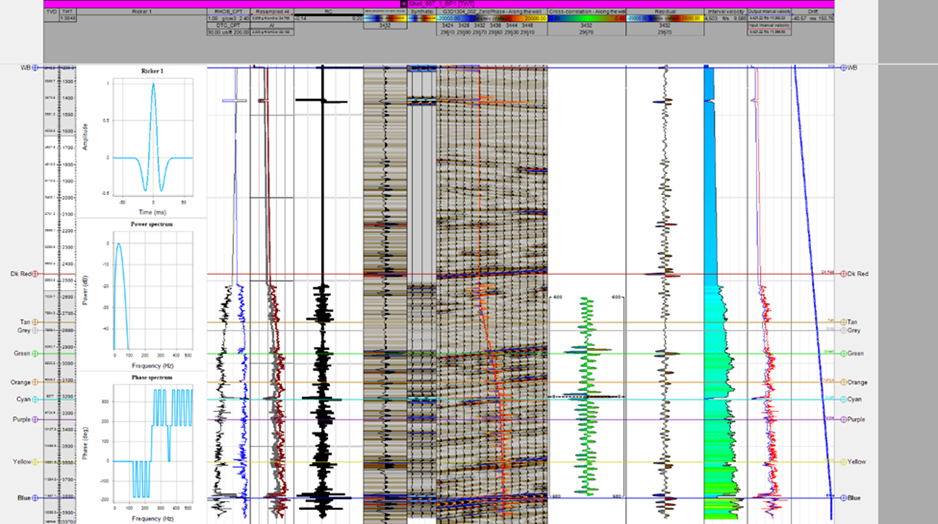
\includegraphics[width=0.75\textwidth]{Images/WellTie Extended.png}
    \caption{This figure shows the seismic-to-well tie demonstrated vy the given key well, well logs, and well tops}
    \label{fig:WellTieZoomed}
\end{figure}

% --- References --- %
\clearpage
\printbibliography

\end{document}
